% !TEX root = Master.tex

After predicting the tree diameter of the LiDAR data, a systematic bias occurs due to the downsides of the LiDAR system difficulties mentioned in Section \ref{Challenges}. To overcome such kind of obstacles of the main goal, i.e. approximating an ideally unbiased diameter distribution of the forest on a compartment level, we introduced a technique which they refer to as "distribution engineering". It takes advantage of some features and diagnostics of parametric distributions. The usefulness of the clusters is also presented in this Section.\\

\begin{figure}[H]
\centering
  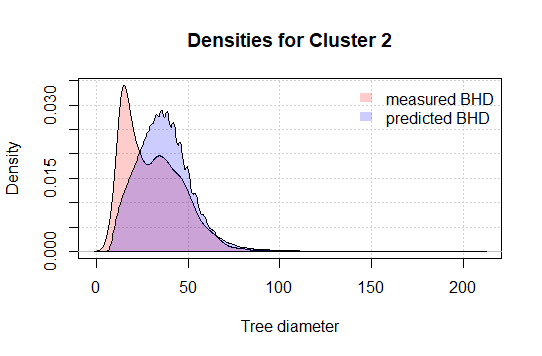
\includegraphics[scale = 0.8]{dens2.png}
  \caption{Measured vs predicted densities of the tree diameter for compartments of the $2^{nd}$ cluster}
  \label{fig:example_dens2}
\end{figure}


In a first step, the diameter values of the LiDAR data as well as the inventory data are subject to a parametric distribution fit. This initial fit is employed on a cluster level, which provides us with the respective parameters of those distributions. In particular but not exclusively, a gamma distribution is fitted in this case (using R-Package: fitdistrplus [16]). The reasoning behind that is to retain coherence, since a GLM gamma regression model was applied to predict the tree diameter. An example for cluster 2 with further details of the fits can be observed in Figure \ref{fig:Fits}.

\begin{figure}[H]
\centering
\begin{subfigure}{.5\textwidth}
  \centering
  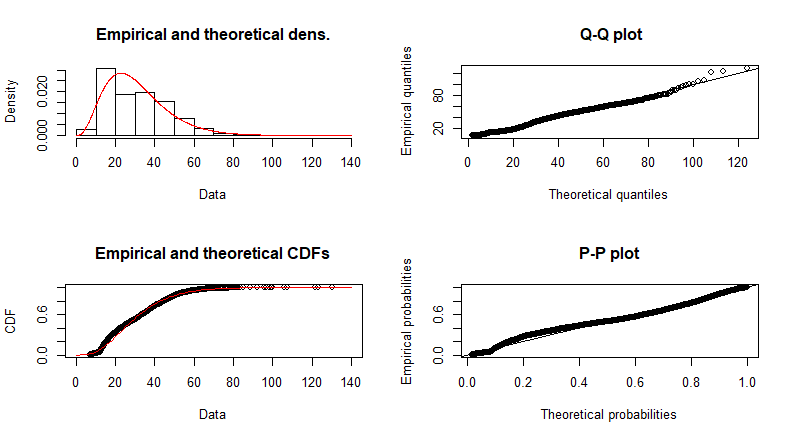
\includegraphics[width=.9\linewidth]{cluster2_valid.png}
  \caption{Inventory}
  \label{fig:cluster2_valid}
\end{subfigure}%
\begin{subfigure}{.5\textwidth}
  \centering
  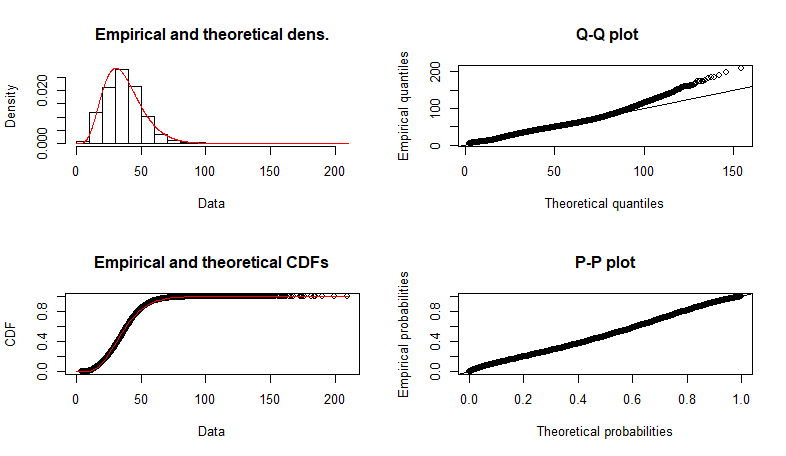
\includegraphics[width=0.85\linewidth]{cluster2_pred.png}
  \caption{LiDAR}
  \label{fig:cluster2_pred}
\end{subfigure}
\caption{Graphical fit diagnostics for cluster 2 - Tree diameter}
\label{fig:Fits}
\end{figure}

Looking at the QQ-Plot of Figure \ref{fig:cluster2_pred}, one can clearly see the outliers of the predicted tree diameter on the upper quanitles (LiDAR), which is (amongst other things) attributed to the overestimation of the crown area discussed previously in Sections \ref{Challenges} \& \ref{Clustering}.\\

The density function of a gamma distribution is composed of a function containing two parameters, the shape parameter $\alpha_{i,j}$ and the rate parameter $\beta_{i,j}$, where $i$ is the cluster index and 
$j$ indicates the data source (Inventory or LiDAR). \\

A summary of the distribution fits can be found in Tables \ref{tab:fitdistrplus_inventory} - \ref{tab:fitdistrplus_lidar}.

\begin{table}[H]
\setlength\arrayrulewidth{1pt}  
\centering
\begin{adjustbox}{max width=\textwidth}
\begin{tabular}{|c|c|c|c|c|c|}
\hline
\rowcolor{Gray}
\textbf{Cluster} & \textbf{Shape} & \textbf{Rate} & \textbf{Log-Likelihood} & \textbf{AIC} & \textbf{BIC} \\ \hline
1                & 6.012          & 0.225        & -20512.63               & 41029.25     & 41042.47     \\ \hline
2                & 3.234          & 0.238         & -1498.457               & 3000.914     & 3008.548     \\ \hline
3                & 3.810          & 0.124         & -17076.31               & 34156.61     & 34169.29     \\ \hline
\end{tabular}
\end{adjustbox}
\caption{Summary of gamma distribution fit on tree diameter of inventory data by MLE}
\label{tab:fitdistrplus_inventory}
\end{table}


\begin{table}[H]
\setlength\arrayrulewidth{1pt}  
\centering
\begin{adjustbox}{max width=\textwidth}
\begin{tabular}{|c|c|c|c|c|c|}
\hline
\rowcolor{Gray}
\textbf{Cluster} & \textbf{Shape} & \textbf{Rate} & \textbf{Log-Likelihood} & \textbf{AIC} & \textbf{BIC} \\ \hline
1                & 9.013          & 0.380         & -4844594                & 9689191      & 9689216      \\ \hline
2                & 4.595          & 0.109         & -122176.7               & 244357.3     & 244373.8     \\ \hline
3                & 5.925          & 0.161         & -17076.31               & 2880304      & 2880325      \\ \hline
\end{tabular}
\end{adjustbox}
\caption{Summary of gamma distribution fit on predicted tree diameter of LiDAR data by MLE}
\label{tab:fitdistrplus_lidar}
\end{table}



This leads to the second step of this procedure, i.e. calculating the correction terms
\begin{align*}
 c_{\alpha_i} = \dfrac{\alpha_{i,invent}}{\alpha_{i,lidar}} \quad \text{and} \quad c_{\beta_i} = \dfrac{\beta_{i,invent}}{\beta_{i,lidar}}
\end{align*}
for every cluster $i$.\\

By multiplying the correction terms with the respective shape and rate parameters of the LiDAR based fit, we obtain the new (corrected) parameters:
\begin{align*}
\alpha^*_i = c_{\alpha_i} * \alpha_{i,lidar} \quad \text{and} \quad \beta^*_i = c_{\beta_i} * \beta_{i,lidar}
\end{align*}
\\

To demonstrate that the corrected parameters return a new and significantly less biased distribution as we would expect, Figures \ref{fig:cluster1_entire_corrected} - \ref{fig:cluster3_entire_corrected} are depicted to compare the old and new densities of the LiDAR diameters with respect to the diameter densities of the inventory. It shall be emphasized that the densities from the inventory data serve as a reference for how the actual densities may look like.

\begin{figure}[H]
\centering
\begin{subfigure}{.5\textwidth}
  \centering
  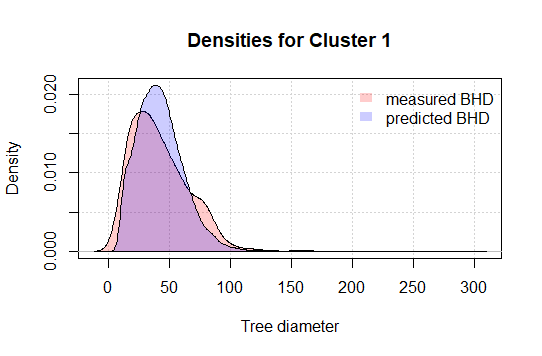
\includegraphics[width=.9\linewidth]{dens1.png}
  \caption{Densities before applying correction terms}
  \label{fig:dens1}
\end{subfigure}%
\begin{subfigure}{.5\textwidth}
  \centering
  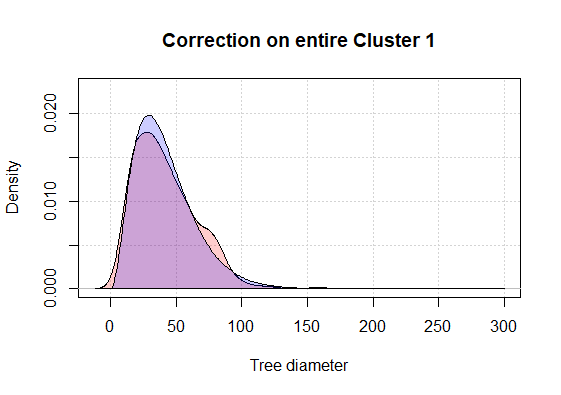
\includegraphics[width=0.843\linewidth]{correction_entire_cluster1.png}
  \caption{Densities after applying correction terms}
  \label{fig:cluster1_pred}
\end{subfigure}
\caption{Measured vs predicted densities of the tree diameter for the $1^{st}$ cluster - Comparison}
\label{fig:cluster1_entire_corrected}
\end{figure}

\begin{figure}[H]
\centering
\begin{subfigure}{.5\textwidth}
  \centering
  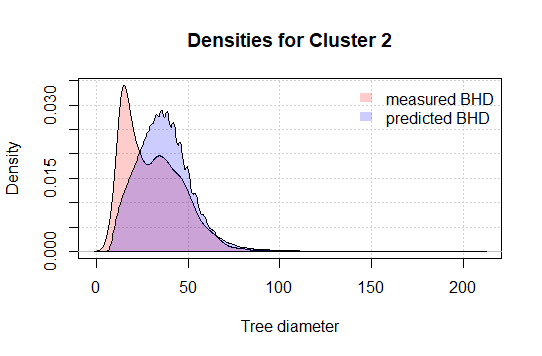
\includegraphics[width=.9\linewidth]{dens2.png}
  \caption{Densities before applying correction terms}
  \label{fig:dens2}
\end{subfigure}%
\begin{subfigure}{.5\textwidth}
  \centering
  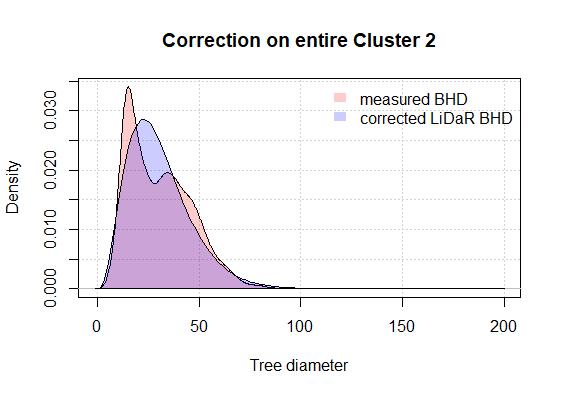
\includegraphics[width=0.845\linewidth]{correction_entire_cluster2.png}
  \caption{Densities after applying correction terms}
  \label{fig:cluster2_pred}
\end{subfigure}
\caption{Measured vs predicted densities of the tree diameter for the $2^{nd}$ cluster - Comparison}
\label{fig:cluster2_entire_corrected}
\end{figure}

\begin{figure}[H]
\centering
\begin{subfigure}{.5\textwidth}
  \centering
  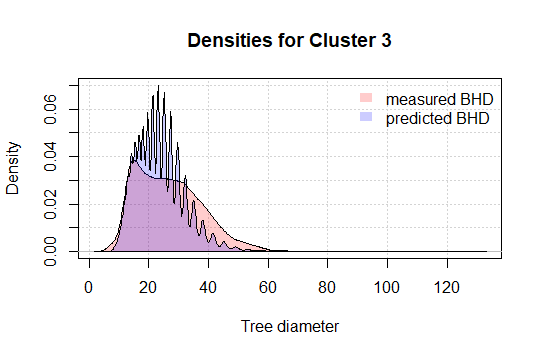
\includegraphics[width=.9\linewidth]{dens3.png}
  \caption{Densities before applying correction terms}
  \label{fig:dens3}
\end{subfigure}%
\begin{subfigure}{.5\textwidth}
  \centering
  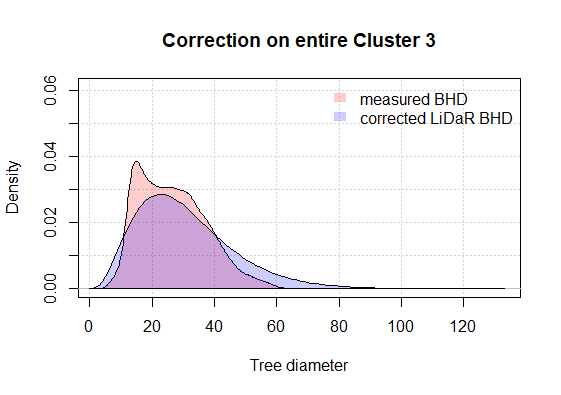
\includegraphics[width=0.842\linewidth]{correction_entire_cluster3.png}
  \caption{Densities after applying correction terms}
  \label{fig:cluster3_pred}
\end{subfigure}
\caption{Measured vs predicted densities of the tree diameter for the $3^{rd}$ cluster - Comparison}
\label{fig:cluster3_entire_corrected}
\end{figure}

Nevertheless, the aim of this technique is to reduce bias on a lower hierarchical level, namely the compartments. Therefore, for every single compartment a gamma distribution is obtained with (corrected) shape and rate parameters 
\begin{align*}
\alpha_{i,k}^* = c_{\alpha_i} * \alpha_{i,k} \quad \text{and} \quad \beta_{i,k}^* = c_{\beta_i} * \beta_{i,k},
\end{align*}
 where $i$ is the cluster allocation of compartment $k$, $\alpha_{i,k}$ and $\beta_{i,k}$ are the shape and rate parameters of the LiDAR based fit on compartment $k$.\\
  Some examples can be seen in Figures \ref{fig:correction_polygon_218a} - \ref{fig:correction_polygon_140a}.

% 218a
\begin{figure}[H]
\centering
\begin{subfigure}{.5\textwidth}
  \centering
  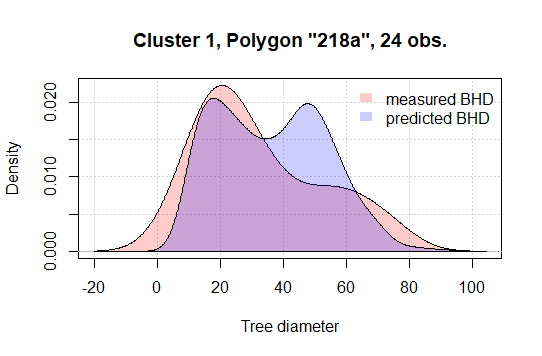
\includegraphics[width=.9\linewidth]{cluster1_218a_24.png}
  \caption{Densities before applying correction terms}
  \label{fig:polygon_before_218a}
\end{subfigure}%
\begin{subfigure}{.5\textwidth}
  \centering
  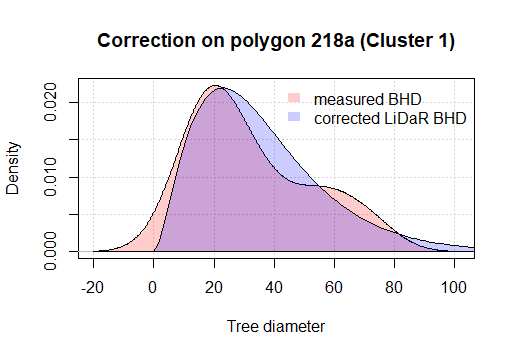
\includegraphics[width=0.86\linewidth]{corrected_cluster1_218a.png}
  \caption{Densities after applying correction terms}
  \label{fig:polygon_after_218a}
\end{subfigure}
\caption{Measured vs predicted densities of the tree diameter for compartment 218a}
\label{fig:correction_polygon_218a}
\end{figure}

% 295a1
\begin{figure}[H]
\centering
\begin{subfigure}{.5\textwidth}
  \centering
  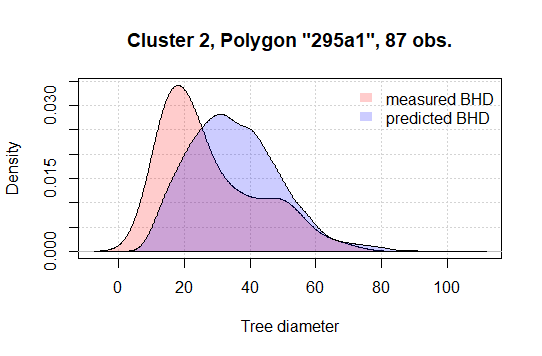
\includegraphics[width=.9\linewidth]{cluster2_295a1_87.png}
  \caption{Densities before applying correction terms}
  \label{fig:polygon_before_295a1}
\end{subfigure}%
\begin{subfigure}{.5\textwidth}
  \centering
  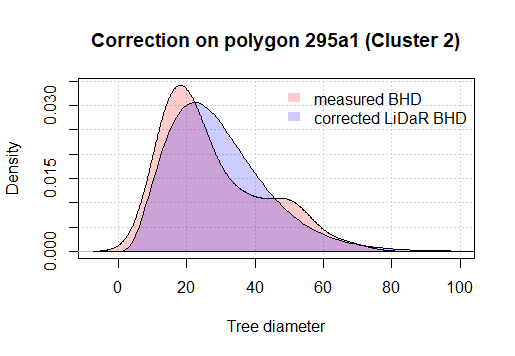
\includegraphics[width=0.853\linewidth]{corrected_cluster2_295a1.png}
  \caption{Densities after applying correction terms}
  \label{fig:polygon_after_295a1}
\end{subfigure}
\caption{Measured vs predicted densities of the tree diameter for compartment 295a1}
\label{fig:correction_polygon_295a1}
\end{figure}

% 275a2
\begin{figure}[H]
\centering
\begin{subfigure}{.5\textwidth}
  \centering
  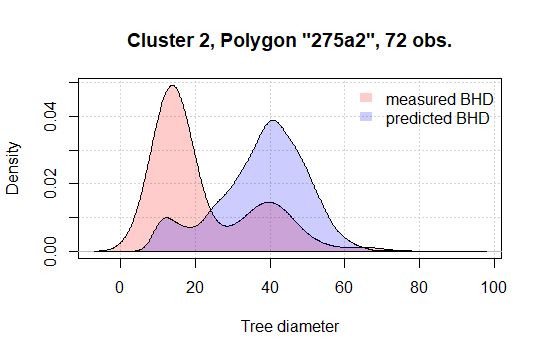
\includegraphics[width=.9\linewidth]{cluster2_275a2_72.png}
  \caption{Densities before applying correction terms}
  \label{fig:polygon_before_275a2}
\end{subfigure}%
\begin{subfigure}{.5\textwidth}
  \centering
  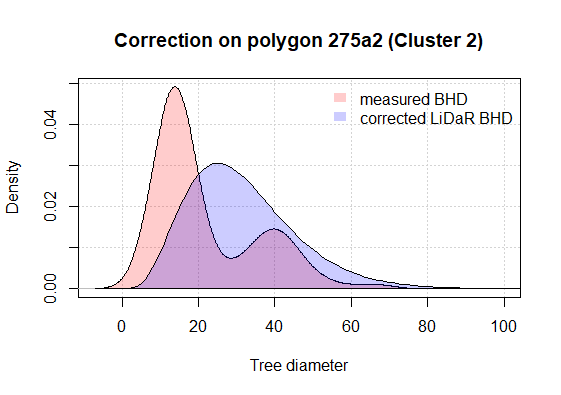
\includegraphics[width=0.837\linewidth]{corrected_cluster2_275a2.png}
  \caption{Densities after applying correction terms}
  \label{fig:polygon_after_275a2}
\end{subfigure}
\caption{Measured vs predicted densities of the tree diameter for compartment 275a2}
\label{fig:correction_polygon_275a2}
\end{figure}

% 140a
\begin{figure}[H]
\centering
\begin{subfigure}{.5\textwidth}
  \centering
  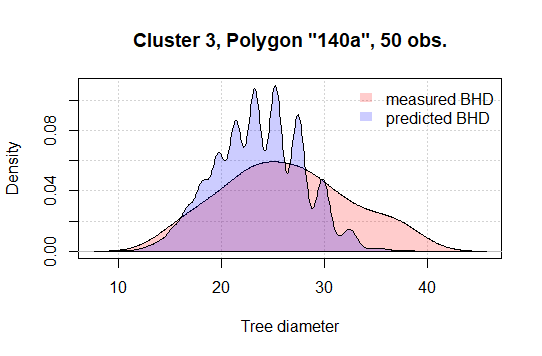
\includegraphics[width=.9\linewidth]{cluster3_140a_50.png}
  \caption{Densities before applying correction terms}
  \label{fig:polygon_before_140a}
\end{subfigure}%
\begin{subfigure}{.5\textwidth}
  \centering
  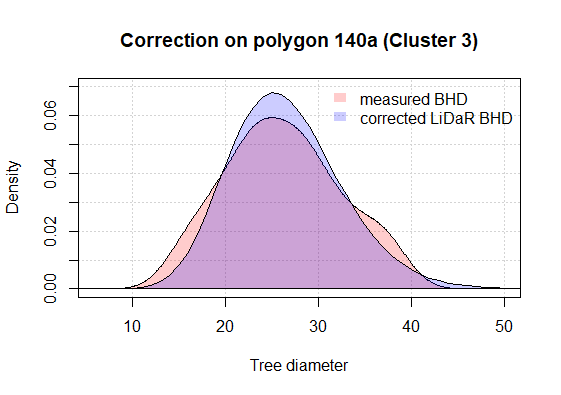
\includegraphics[width=0.835\linewidth]{corrected_cluster3_140a.png}
  \caption{Densities after applying correction terms}
  \label{fig:polygon_after_140a}
\end{subfigure}
\caption{Measured vs predicted densities of the tree diameter for compartment 140a}
\label{fig:correction_polygon_140a}
\end{figure}

Advantageously, corrected diameter densities from LiDAR data can be estimated even if there was no sampling carried out on a specific compartment. All that is needed is the compartment's allocation to a certain cluster. Another resolved issue using this method is that the corrected densities do no longer show long tails, meaning that overestimation is dealt with efficiently.